
\chapter{Anwendung und Algorithmus}

Ziel dieser Arbeit ist es nicht nur eine Methodik zur optische 
Deformationserkennung zu entwickeln, sondern diese Methodik auch in einer 
Anwendung einfach nutzbar zu machen. 

Diese Kapitel dokumentiert diese Anwendung und geht auf Herausforderungen 
in der Entwicklung ein.

\section{Anwendung}

Die Anwendung beinhaltet verschiedene Funktionen, alle Funktionen 
können separat benutzt werden. Dadurch müssen zeitintensive Vorgänge nicht 
wiederholt werden, sondern Zwischenergebnisse können abgespeichert und 
neu geladen werden.
Die Anwendung bietet Funktionen, um Resultate in dem entsprechenden Dateiformat zu 
speichern. Soweit möglich werden Dateinamen Empfehlungen automatisch ermittelt, 
daher ist es zu empfehlen von Anfang an mit einem einheitlichen Namensschema bei
den 3D-Scannerdaten zu arbeiten. 
Das Schema \glqq Bauteilbeschreibung \textunderscore Spannungsstufe\grqq~~
\textunderscore Scannerdurchlauf.ply
wird empfohlen. Ein Beispiel für die zweite Pointcloud eines FDM-Bauteil bei der
vierten Spannungsstufen wäre also \glqq FDM0\textunderscore SP4\textunderscore 2.ply\grqq~.
In Abbildung \ref{fig:software_screenshot} ist die Oberfläche der Anwendung zu sehen.

\begin{figure}[H]
    \centering
    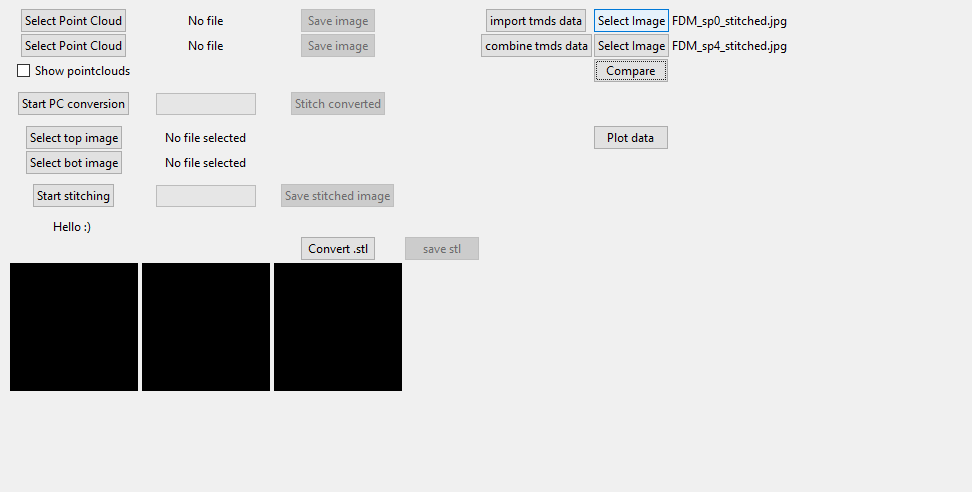
\includegraphics[width=0.9\textwidth]{images/software_screenshot.png}
    \caption{Anwendungsoberfläche}
    \label{fig:software_screenshot}
\end{figure}

Über die Buttons \glqq Select Pointcloud\grqq~ können Pointclouds zum Konvertieren in Bilder
ausgewählt werden. Der Text neben dem Bild zeigt den Dateinamen der ausgewählten 
Datei an. Die obere Pointcloud sollte hier als erstes ausgewählt werden.
Der Button \glqq Start PC conversion\grqq~~startet die Konvertierung. Der Balken 
daneben zeigt den Prozessfortschritt. 
Wenn \glqq Show Pointclouds\grqq~ gesetzt ist, werden die Pointclouds vor dem 
Konvertieren in einem separaten Fenster angezeigt. So kann überprüft werden, ob die 
korrekte Pointcloud ausgewählt wurde.
Wenn der Prozess abgeschlossen ist, werden die resultieren Bilder als Vorschau in der 
Anwendung angezeigt und die Option zum Speichern der Bilder ist nicht mehr ausgegraut.
Zusätzlich wird nach dem Konvertierungsprozess die Schaltfläche 
\glqq Stitch converted\grqq~ freigeschaltet. Durch diese Option können die 
Bilder direkt zusammengefügt werden, ohne das die Bilder extra gespeichert und 
eingeladen werden müssen. Wenn schon existierende Bilder zusammengefügt werden sollen, 
können die Schaltflächen \glqq Select top image\grqq und \glqq Select bot image\grqq
ausgewählt werden um das obere und untere Bild auszuwählen. Auch hier wird die 
ausgewählte Datei als Text angezeigt. Die Dateiauswahl erfolgt über das 
Windows-Kontextmenü, der zuletzt verwendete Ordner wird hierbei erhalten, sodass das 
zweite Bild schneller ausgewählt werden kann. 
Über den Button \glqq Start stitching\grqq wird der stitching Prozess gestartet. 
Auch hier wird der Fortschritt und das Endresultat, sobald es vorliegt, angezeigt.

Damit auch die CAD-Datei des additiv gefertigten Bauteils verglichen werden kann, 
existiert der \glqq Convert stl\grqq~ Button. Hier wird eine .stl Datei zu einem Bild 
konvertiert und kann über \glqq save stl\grqq~ gespeichert werden.

Mithilfe der rechts zu sehenden Schaltflächen können Bilder auf ihre Deformation hin 
verglichen werden. Die resultieren Deformationsdaten werden automatisch als Textdatei
in dem Ordner \glqq deformation\underline data\grqq~ gespeichert. Dieser Ordner wird automatisch 
in dem Verzeichnis erzeugt, in dem die Anwendung ausgeführt wird. 
Die erstellten Textdateien können mithilfe des Buttons \glqq Plot data\grqq~ ausgewählt 
werden, und werden automatisch als Graph angezeigt. 

Beim Konvertieren und stitchen werden alle Prozesse, die nicht voneinander abhängig sind,  
nebenläufig ausgeführt. Das reduziert die Laufzeit der Prozesse.

Die Anwendung ist in Python geschrieben, rechenintensive Prozesse wurden aber mithilfe 
der Bibliothek \glqq Numba\grqq~in optimierten Maschinencode compiliert~\cite{numba}.
Dadurch ist der Konvertierungs- und Stitching-Prozess deutlich schneller geworden. 
Durch die Optimierungen konnte der Konvertierungsprozess von 49 s auf 41 s verschnellert 
werden. Bei dem Stitchprozess war die Verbesserung noch deutlicher. Hier 
beträgt die Laufzeit mit Optimierungen ca. 30 s um zwei Konturen zu vergleichen. 
Ohne Optimierungen braucht der Vergleich derselben beiden Konturen 
hochgerechnet 600 Minuten.



